\picdata=['21', '5']TKS01000['Tri-3.tex', '2']
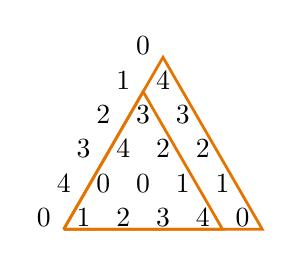
\begin{tikzpicture}
[scale=0.504528]
\node at (0.000000,0.000000) {0};
\node at (1.000000,-0.000000) {1};
\node at (0.500000,0.866025) {2};
\node at (0.000000,1.732051) {3};
\node at (-0.500000,0.866025) {4};
\node at (-1.000000,0.000000) {0};
\node at (-1.500000,-0.866025) {1};
\node at (-0.500000,-0.866025) {2};
\node at (0.500000,-0.866025) {3};
\node at (1.500000,-0.866025) {4};
\node at (2.500000,-0.866025) {0};
\node at (2.000000,-0.000000) {1};
\node at (1.500000,0.866025) {2};
\node at (1.000000,1.732051) {3};
\node at (0.500000,2.598076) {4};
\node at (0.000000,3.464102) {0};
\node at (-0.500000,2.598076) {1};
\node at (-1.000000,1.732051) {2};
\node at (-1.500000,0.866025) {3};
\node at (-2.000000,0.000000) {4};
\node at (-2.500000,-0.866025) {0};
\draw[orange!90!black,line width=1] (-2.000000,-1.154701)  -- (-2.000000,-1.154701)  -- (2.000000,-1.154701)  -- (0.000000,2.309401)  -- (-2.000000,-1.154701);
\draw[orange!90!black,line width=1] (-2.000000,-1.154701)  -- (-2.000000,-1.154701)  -- (3.000000,-1.154701)  -- (0.500000,3.175426)  -- (-2.000000,-1.154701);
\end{tikzpicture}

